\documentclass[10pt,twocolumn,letterpaper]{article}

\usepackage{cvpr}
\usepackage{times}
\usepackage{epsfig}
\usepackage{graphicx}
\usepackage{amsmath}
\usepackage{amssymb}

% Include other packages here, before hyperref.

% If you comment hyperref and then uncomment it, you should delete
% egpaper.aux before re-running latex.  (Or just hit 'q' on the first latex
% run, let it finish, and you should be clear).
\usepackage[breaklinks=true,bookmarks=false]{hyperref}

\cvprfinalcopy % *** Uncomment this line for the final submission

\def\cvprPaperID{****} % *** Enter the CVPR Paper ID here
\def\httilde{\mbox{\tt\raisebox{-.5ex}{\symbol{126}}}}

% Pages are numbered in submission mode, and unnumbered in camera-ready
%\ifcvprfinal\pagestyle{empty}\fi
\setcounter{page}{1}
\begin{document}

%%%%%%%%% TITLE
\title{Semantic Segmentation of Urban Scenes using Encoder-Decoder Architecture}

\author{Zheng Luo\\
Department of Computer Science\\
University of Virginia\\
{\tt\small zl5sv@virginia.edu}
% For a paper whose authors are all at the same institution,
% omit the following lines up until the closing ``}''.
% Additional authors and addresses can be added with ``\and'',
% just like the second author.
% To save space, use either the email address or home page, not both
%\and
%Zixuan Lin\\
%Department of Biomedical Engineering\\
%University of Virginia\\
%{\tt\small zl7qk@virginia.edu}
}

\maketitle
%\thispagestyle{empty}

%%%%%%%%% ABSTRACT
\begin{abstract}
   Autonomous vehicles are assumed to be the key units of the next generation transportation system. Since vehicle safety is critical to real world, it is important to maintain that a vehicle’s understanding to environment is highly reliable. Real-world driving environment is a mixture of multiple objects, and can be dense especially on urban roads. Vehicles are assumed to not only recognize multiple objects in the whole scene but also know where exactly different objects occupy. Therefore, while cameras are widely used to recognize objects, image segmentation (or clustering pixels) from a mixture becomes the challenge at the first step, in order to understand the environment precisely.
\end{abstract}




%%%%%%%%% BODY TEXT
\section{Introduction}

In this project, the plan is to cast existing different neural networks and fine tune them to segment the validation sets in Cityscapes Dataset. Finding a proper way to modify the network structures is the first important task. Moreover, we will find fine annotated training sets to train convolutional neural networks. Except playing different neural networks and compare (and try to improve) their performance of segmentation and recognition, another experiment can also be planned to test the adaptivity of trained neural networks. That is, the project is also able to study if a fine-tuned network for a single city can behave well on images from another city. Alternatively speaking, if the training set is a mixture of many different cities, it is interesting to know how much improvement can be achieved compared to only using a single or few cities.

\begin{figure}[t]
\centering
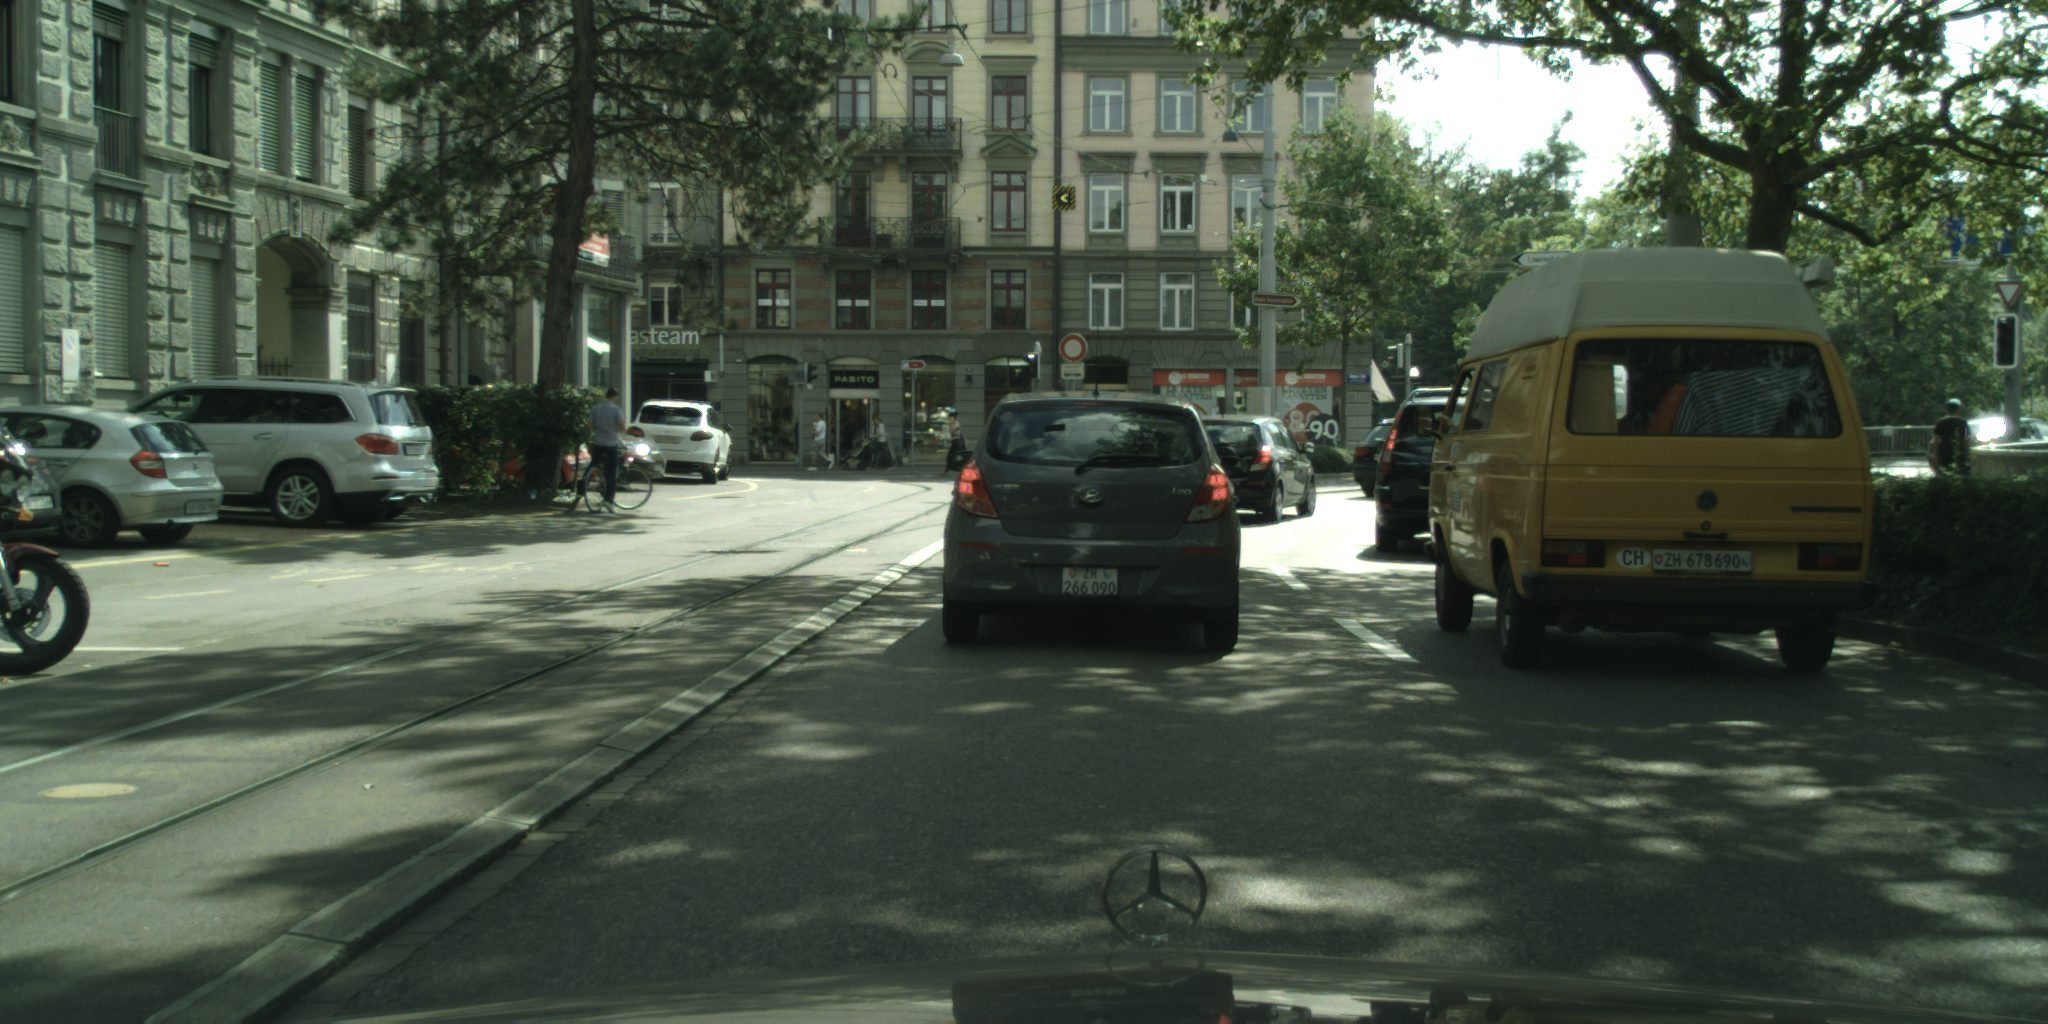
\includegraphics[width=0.40\textwidth]{zurich_example.png}
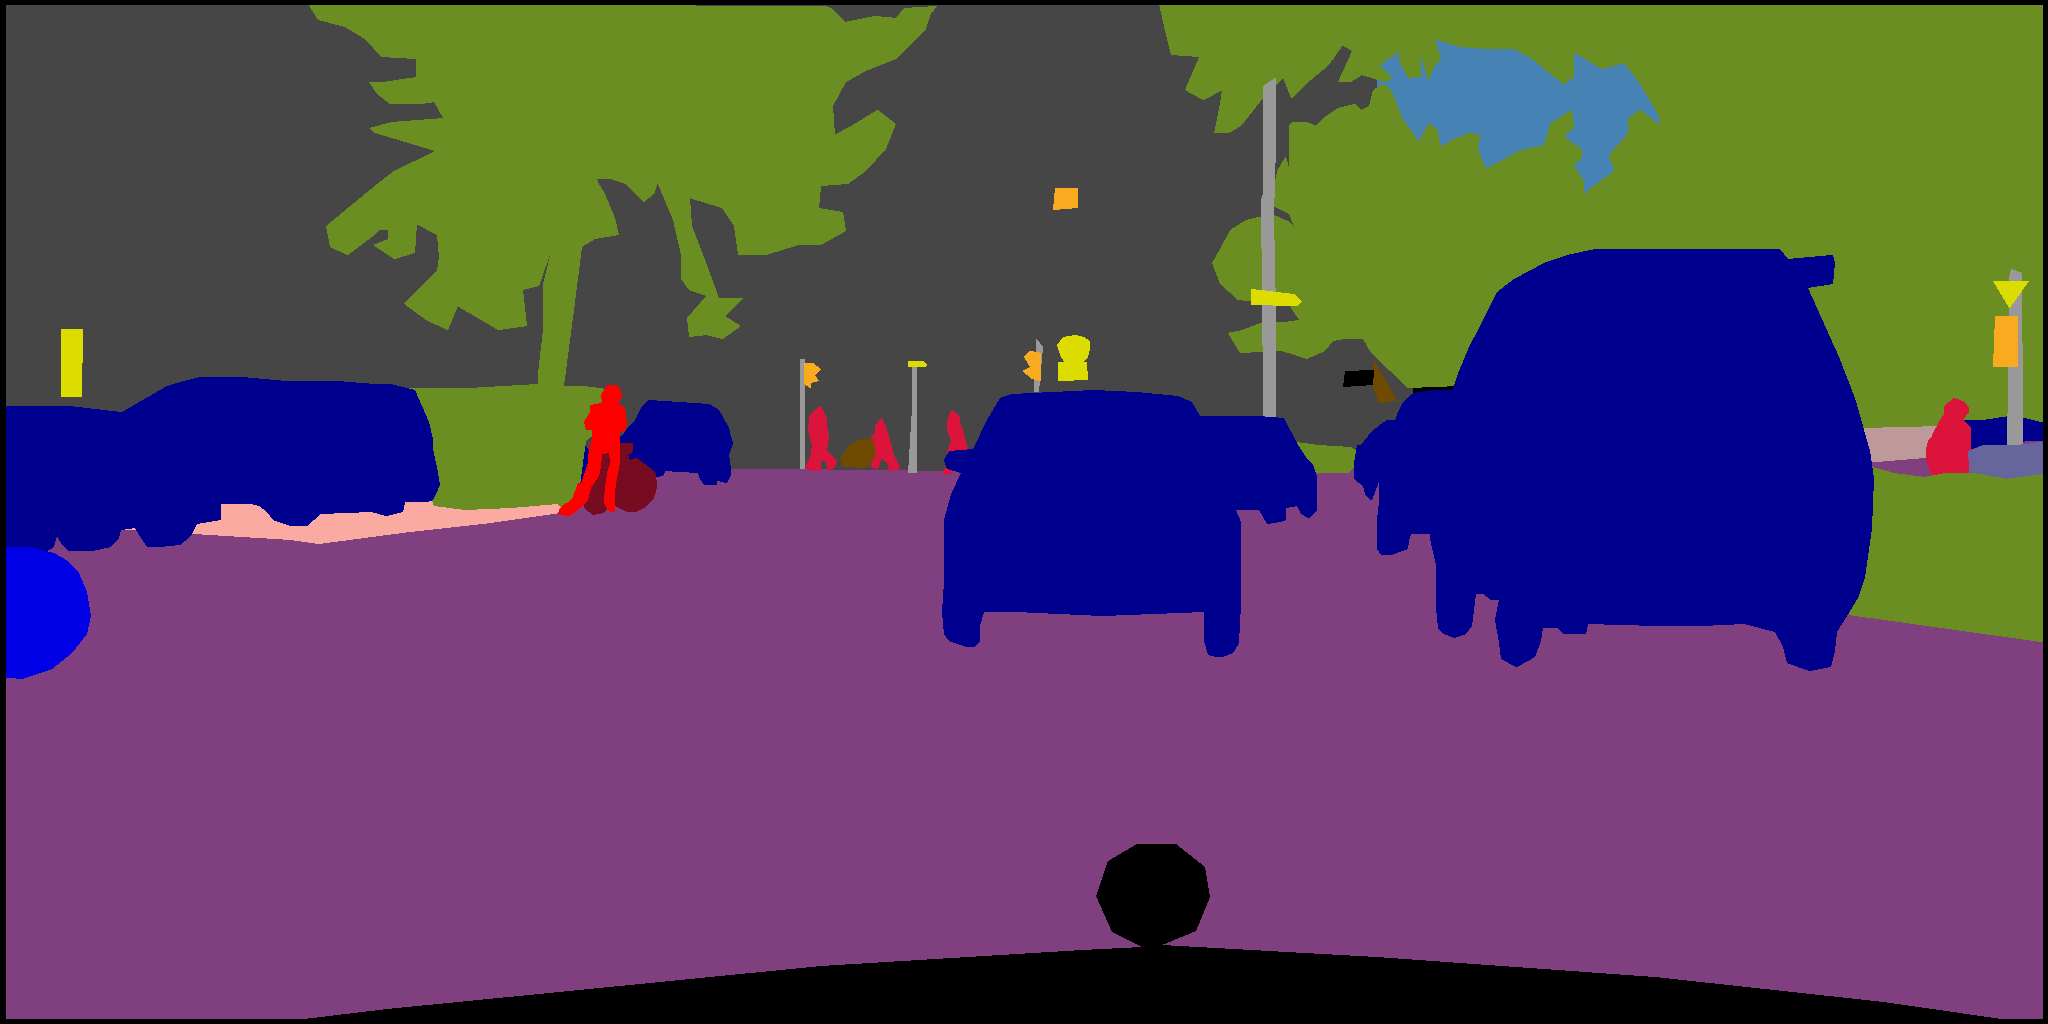
\includegraphics[width=0.40\textwidth]{zurich_example_seg.png}
\caption{Here is an illustration of fine annotated urban scene from Cityscapes Dataset. The upper side is an original image with 2048$\times$1024 resolution taken from Zuerich. The bottom side is its corresponding fine annotation. The overlayed color represents semantic classes defined by the dataset provider.}
\label{fig:leadfigure}
\end{figure}

\section{Related Work}
Proven classification architectures such as AlexNet and VGG (and their successors) are widely used for single-object recognitions. However, segmentation requires pixel-wise output to distinguish different objects rather than a single judgement. In 2015, Long et al. \cite{Long_2015_CVPR} introduced fully convolutional networks to adapt those classifiers for dense prediction, with in-network up-sampling and a pixel-wise loss. Therefore, by converting and fine tuning currently existing convolutional neural networks, it is possible to achieve a much better performance of segmentation than other simple methods such as k-means clustering and watershed transform.

Since this project is going to play a role among the problems of autonomous driving, Cityscapes Dataset \cite{Cordts2016Cityscapes} will be used in this project. It has fine annotated images and more coarse annotated images of urban scenarios from multiple cities. We will firstly use the 5000-image volumn including 3475 pixel-level fine annotated images for training and validation, and 1525 dummy annotated images for testing. The dummy annotation means regions are ignored. Class labels are defined and also grouped semantically. This dataset can be very useful due to its high quality and images resources (multiple cities). The dataset also have benchmarks for pixel-level and instance-level semantic labeling. They can be used to show segmentation performance quantitatively.


%-------------------------------------------------------------------------
\section{Model Structure}
VGG-16 \cite{Simonyan14c} has an outstanding performance on many datasets such as ImageNet for purposes of object recognition. Although casting VGG-16 to a fully convolutional network in the way described by \cite{Long_2015_CVPR} does handle the task for image segmentation, the resolution of segmentation is not good enough even if the training input has high resolutions. Therefore, we cast VGG-16 to an FCN with combinations of upsampling (unpooling) and convolutional layers (decoders) appended after convolutional layers, by following the method described in \cite{badrinarayanan2015segnet2}. This architecture is named SegNet which contains an encoder followed by a decoder. Intuitively, we can consider the encoder part is responsible for feature extraction while the decoder handles the task of transforming deep features to RGB space.

\subsection{Network Structure}
First of all, we follow the structure of VGG-16 with batch normalization \cite{ioffe2015batch} but simply discard the fully connected layers of it. Then, we append a set of unpooling and convolutional layers with batch normalization symmetrically to the encoder part, but with the output channel equal to the number of classes for the last layer. At the end of the network, we add a softmax function to produce class predictions for each pixel in the input image. That is, for each pixel, the network will give a probability distribution telling the likelihood of belonging to each class. This is an analog to the case of image classification, but is actually performing pixel-wise classifications. The detailed structure is showing as Figure 2.

\begin{figure}[h]
	\centering
	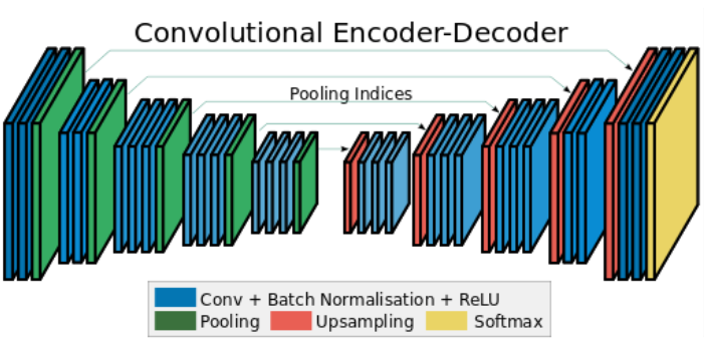
\includegraphics[width=0.40\textwidth]{model.png}
	\caption{Here is the encoder-decoder architecture used for this pixel-level semantic labeling/segmentation task. It is introduced in \cite{badrinarayanan2015segnet2} and named as SegNet. The architecture uses un-pooling instead of de-convolutional layers for tensor up-scaling.}
	\label{fig:model}
\end{figure}

In addition, we also add $``$links$"$ between each corresponding pooling and unpooling layers. This means the unpooling layers are deterministic with respect to max-pooling layers. When data goes through pooling layers, we record the indices of preserved pixels (or tensor elements). When doing unpooling, we place tensor elements back to the same places according to the previously recorded indices.

Therefore, the image input to the network is a tensor of size B$\times$C$\times$H$\times$W while the label (mask) input to it is a tensor of size B$\times$H$\times$W, where B, C, W, H stand for batch size, number of channels, image width, and image height respectively. The output of the network is a tensor of size B$\times$N$\times$H$\times$W where N stands for number of classes.

\subsection{Loss Function}
The loss function for this segmentation purpose is 2D cross-entropy loss. The idea is the same as the case of image classifications. Let P be the output (predictions) of the network, and have size N$\times$H$\times$W, and M of size H$\times$W be the ground-truth label of the segmented image; then the loss is defined as the following:
\begin{center}
	$Loss = -\sum_{i=0}^{W}\sum_{j=0}^{H}logP(M(j,i),j,i).$
\end{center}
With this loss function, we use Adam to train the network with learning rate $2\times10^{-4}$, weight decay $1\times10^{-4}$, and all other settings default in Pytorch.

\section{Experiments}
When training the network defined above, we use about 3100 fine-annotated images as the training set and the rest about 100$\sim$200 fine-annotated images as the validation set, while the actual number varies since different cities have different numbers of images. We have written a dataloader for CityScapes that can handle the whole fine-annotated dataset, including image transformations. There are also a fine-annotated test set but the ground-truth labels are only available on the server of Cityscapes website. Therefore, this test set is not used for our experiments.

The experiments break down into two main parts which will be described in this section. The first part is to train the network on a set of cities and validate it on another city that is exactly not included in the training set. The second part is to train a network among all of cities and validate it on the same set of cities, where training set and validation set are always mutual exclusive. The purpose of this experimental design is to explorer the adaptivity of neural networks with different prior knowledge. The details of dataset content are shown in Table 1.

\begin{table}[h]
\begin{center}
	\begin{tabular}{ | l | p{4.6cm} | }
		\hline
		Germany & Aachen(174) Bochum(96) Bremen(316) Cologne(154)
		Darmstadt(85) Dusseldorf(221) Erfurt(109) Frankfurt(267) Hamburg(248) Hnaover(196) Jena(119) Krefeld(99) Lindau(59) Monchengladbach(94) Munster(174) Stuttgart(196) Tubingen(144) Ulm(95) Weimar(142)\\ \hline
		France & Strasbourg(365)\\ \hline
		Switzerland & Zurich(122)\\
		\hline
	\end{tabular}
\end{center}
\caption{The set of cities, their countries, and the number of corresponding images available in the fine-annotated dataset.} \label{tab:table1}
\end{table}

\subsection{Dataset Modifications}
As mentioned in \cite{Cordts2016Cityscapes}, only 19 classes frequently appear in those images, therefore the benchmark will only consider those 19 classes to avoid ambiguity. In this project, we discard labels other than the 19 classes by setting those discarded labels to the same value 255. When doing segmentation, those classes will be considered as the same $``$unknown$"$class.

Since the images in the dataset have a high resolution (2048$\times$1024), we resize them to 256$\times$128 in order to save time and graphic memories. When resizing the images, we use the default bicubic method. When resizing the masks (labels), we use nearest neighbors.

\subsection{Training on All Cities}
First of all, we train a network on all cities. The validation set is composed by taking 12 images out from each city. We train it for 10 epochs with batch size 7. This will be the baseline for further comparison. The training curve and sample result (an image from Frankfurt) are shown in Figure 3.

\subsection{Training without Strasbourg}
Since we want to explore the adaptivity of the network, we try to maximize the potential difference on the training set and validation set. To do this, we train the network on cities only from Germany and Switzerland and validate it on Strasbourg which is a city of France. Again, the network is trained for 10 epochs with batch size 7. The training curve and sample result (an image from Strasbourg) are shown in Figure 4.

\subsection{Training without Zurich}
Similar to the previous case, we take out Zurich of Switzerland, and train the network on cities from Germany and France. We still set the batch size to be 7 and train the network for 10 epochs. The training curve and sample result (an image from Zurich) are shown in Figure 5.

\begin{figure}[h]
	\centering
	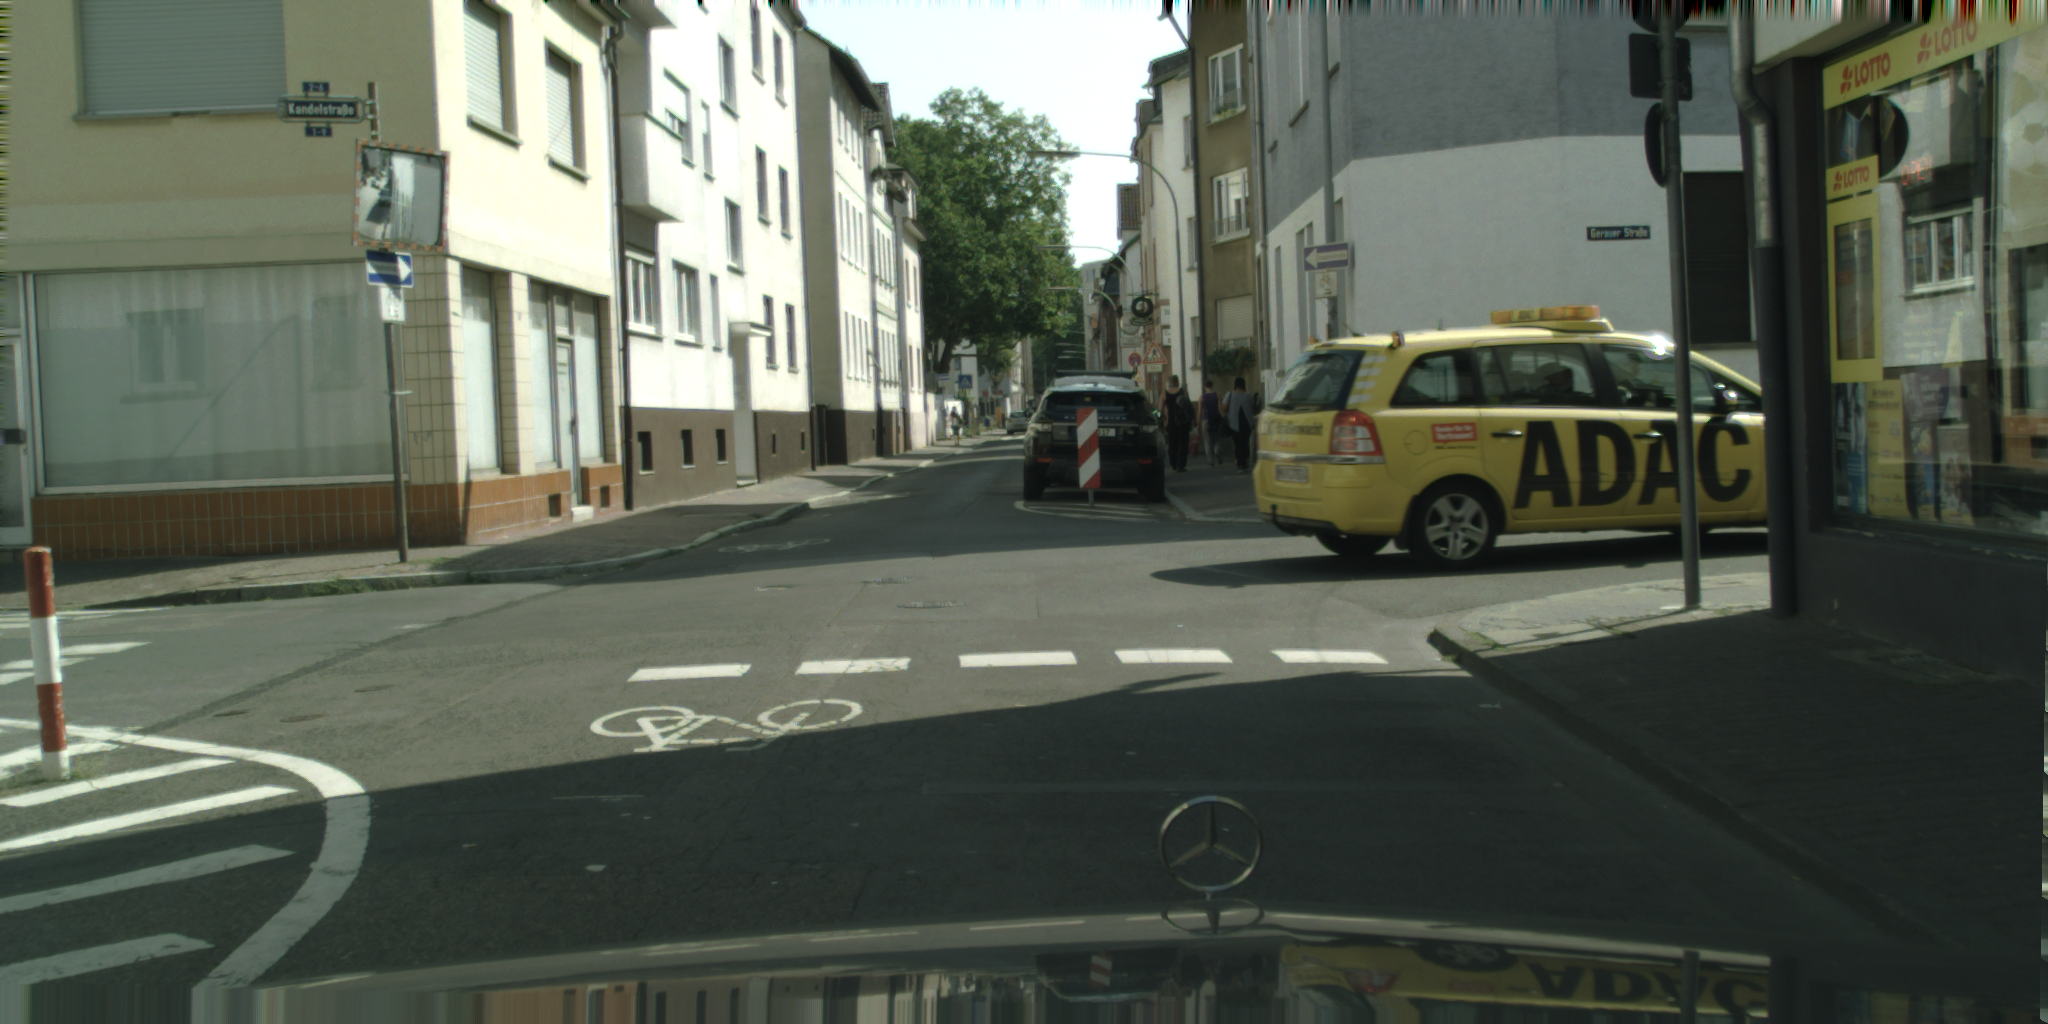
\includegraphics[width=0.23\textwidth]{frankfurt.png}
	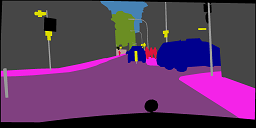
\includegraphics[width=0.23\textwidth]{frankfurt_gt.png}
	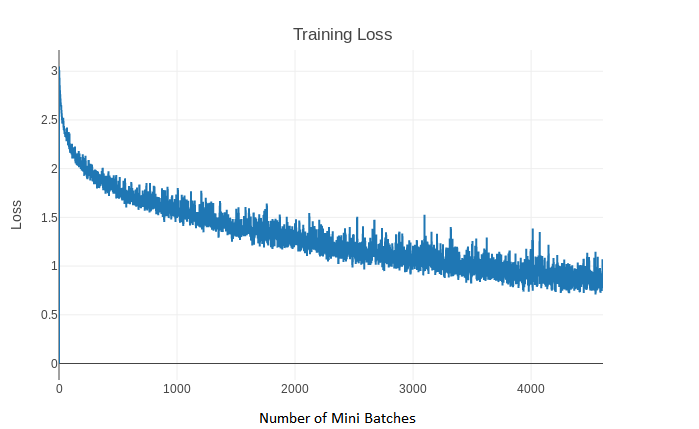
\includegraphics[width=0.23\textwidth]{curve_all.png}
	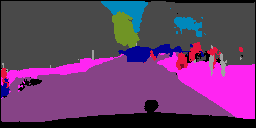
\includegraphics[width=0.23\textwidth]{frankfurt_seg.png}
	\caption{Top left: input image; top right: ground truth; bottom left: training curve; bottom right: segmentation result.}
	\label{fig:figure2}
\end{figure}

\begin{figure}[h]
	\centering
	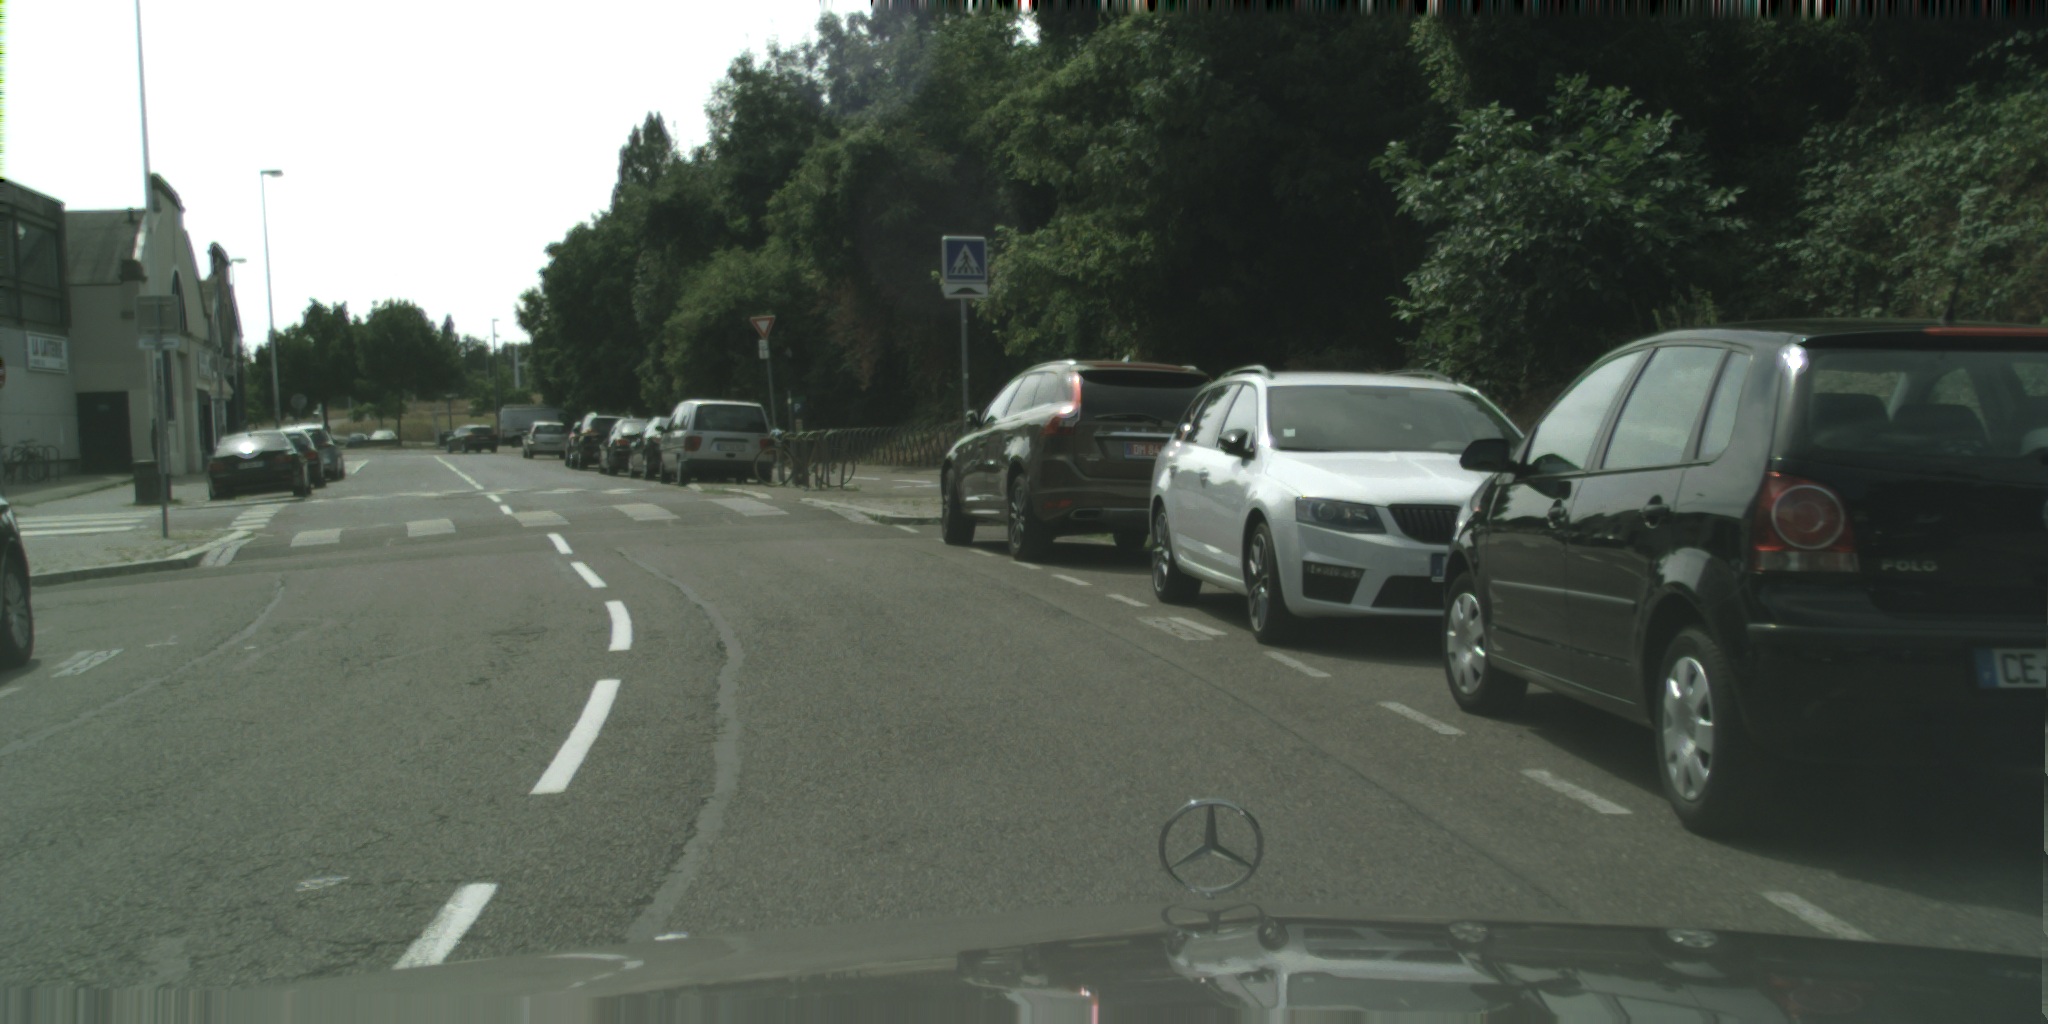
\includegraphics[width=0.23\textwidth]{strasbourg.png}
	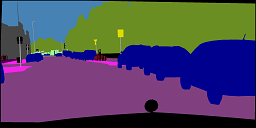
\includegraphics[width=0.23\textwidth]{strasbourg_gt.png}
	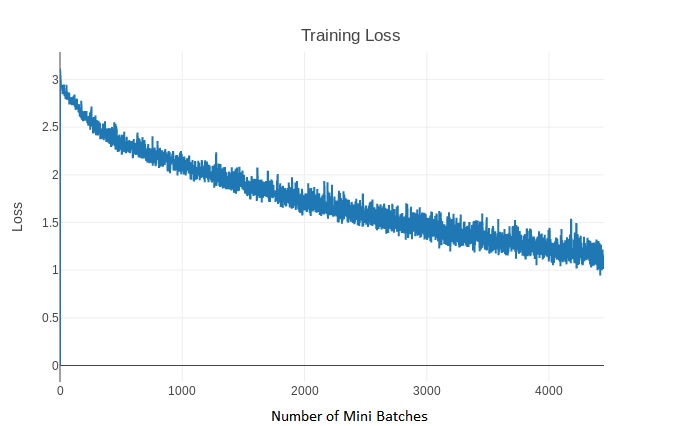
\includegraphics[width=0.23\textwidth]{curve_without_strasbourg.png}
	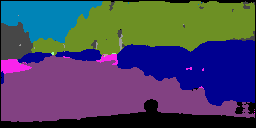
\includegraphics[width=0.23\textwidth]{strasbourg_seg.png}
	\caption{Top left: input image; top right: ground truth; bottom left: training curve; bottom right: segmentation result.}
	\label{fig:figure3}
\end{figure}

\begin{figure}[h]
	\centering
	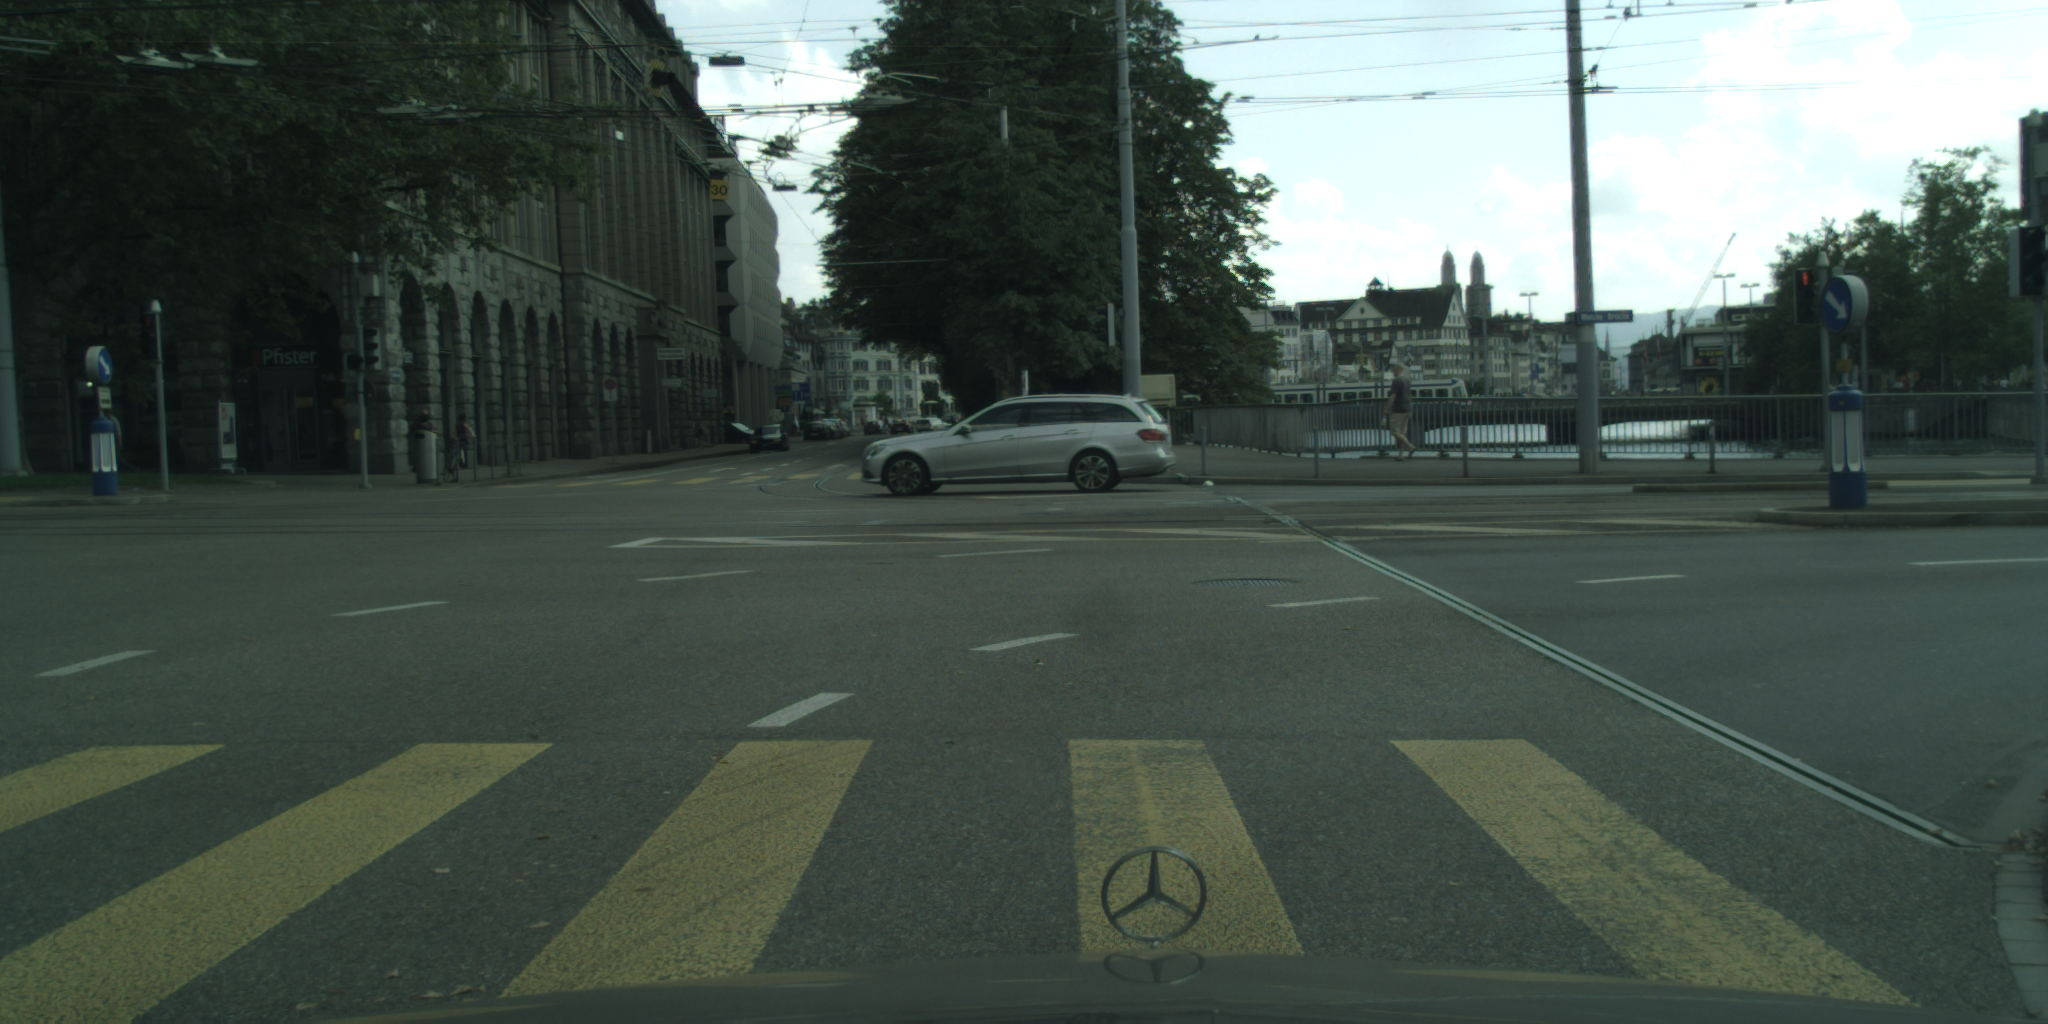
\includegraphics[width=0.23\textwidth]{zurich.png}
	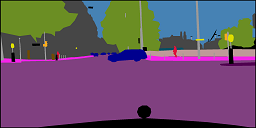
\includegraphics[width=0.23\textwidth]{zurich_gt.png}
	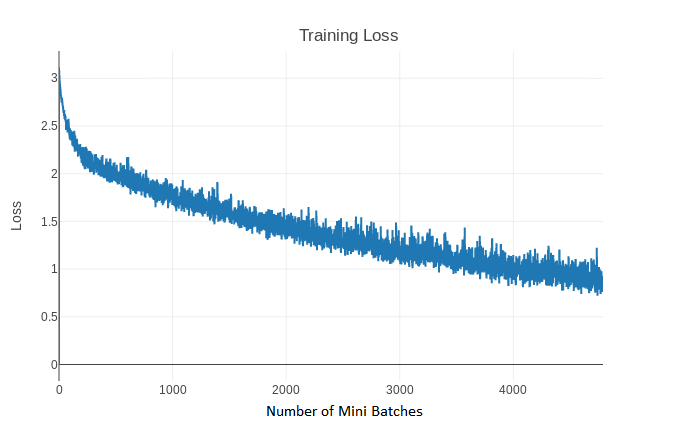
\includegraphics[width=0.23\textwidth]{curve_without_zurich.png}
	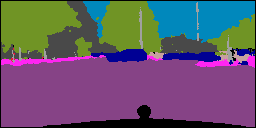
\includegraphics[width=0.23\textwidth]{zurich_seg.png}
	\caption{Top left: input image; top right: ground truth; bottom left: training curve; bottom right: segmentation result.}
	\label{fig:figure4}
\end{figure}

\subsection{Results Comparison}
The benchmark for pixel-level semantic labeling task is called intersection-over-union (IoU) metric from PASCAL VOC \cite{everingham2015pascal}. It is defined as
\begin{center}
	$IoU=\dfrac{TP}{TP+FP+FN}$
\end{center}
where TP, FP, and FN are the numbers of true positive, false positive, and false negative pixels respectively.

\begin{table}[h]
	\begin{center}
		\begin{tabular}{ | l | p{2cm} | }
			\hline
			Model & Mean IoU\\ \hline \hline
			Training on All Cities & 0.3167\\ \hline
			Training without Strasbourg & 0.2937\\ \hline
			Training without Zurich & 0.3086\\
			\hline
		\end{tabular}
	\end{center}
	\caption{The left column indicates the models and validation sets corresponding to Section 4.2, 4.3, and 4.4; the right column shows the mean IoU values from their validation.} \label{tab:table2}
\end{table}

We show the mean IoU values for each model we trained on their corresponding validation sets in Table 2. The results show that the first model has a slightly better performance as it is trained with full information.

\section{Conclusion and Future Work}
Training a neural network is actually encoding deep features from input data into a large nonlinear function. Therefore, dataset is significant for the performance of the trained network since network inference relies on the implicit information learned from the dataset. From this point of view, we can analyze the adaptivity of the trained network with respect to the training set. In this project, to some extent, the benchmark results do imply that inference performance will be better if the network can obtain the full information from the dataset. The difference is quite small since street views in Europe cities can be very similar.

\subsection{Unbalanced and Limited Dataset Size}
On the other hand, we are not very confident about the above conclusion due to the very small performance gap. As we can see in Table 1, the numbers of images for different cities can be largely different (e.g. 122 for Zurich and 365 for Strasbourg). Therefore, the results (mean IoU values) could be biased due to the different statistics of objects in the images.

\subsection{Data Augmentation}
Fine annotation for such an image segmentation purpose requires a lot of human efforts. Therefore, the size of the dataset is not large especially compared to datasets for image classification. As shown in Figure 6, in this project, if we use the network trained by down-sampled images and labels and test it using a full size image, segmentation results will be much worse. The reason could be that some detailed information vanishes during down-sampling. Therefore, instead of resizing the training inputs, we can perform uniformly random crops to the large images to save graphic memories. Ideally, as the number of training epochs increase, the network should gain full information/features as inputing full-size images.

\begin{figure}[h]
	\centering
	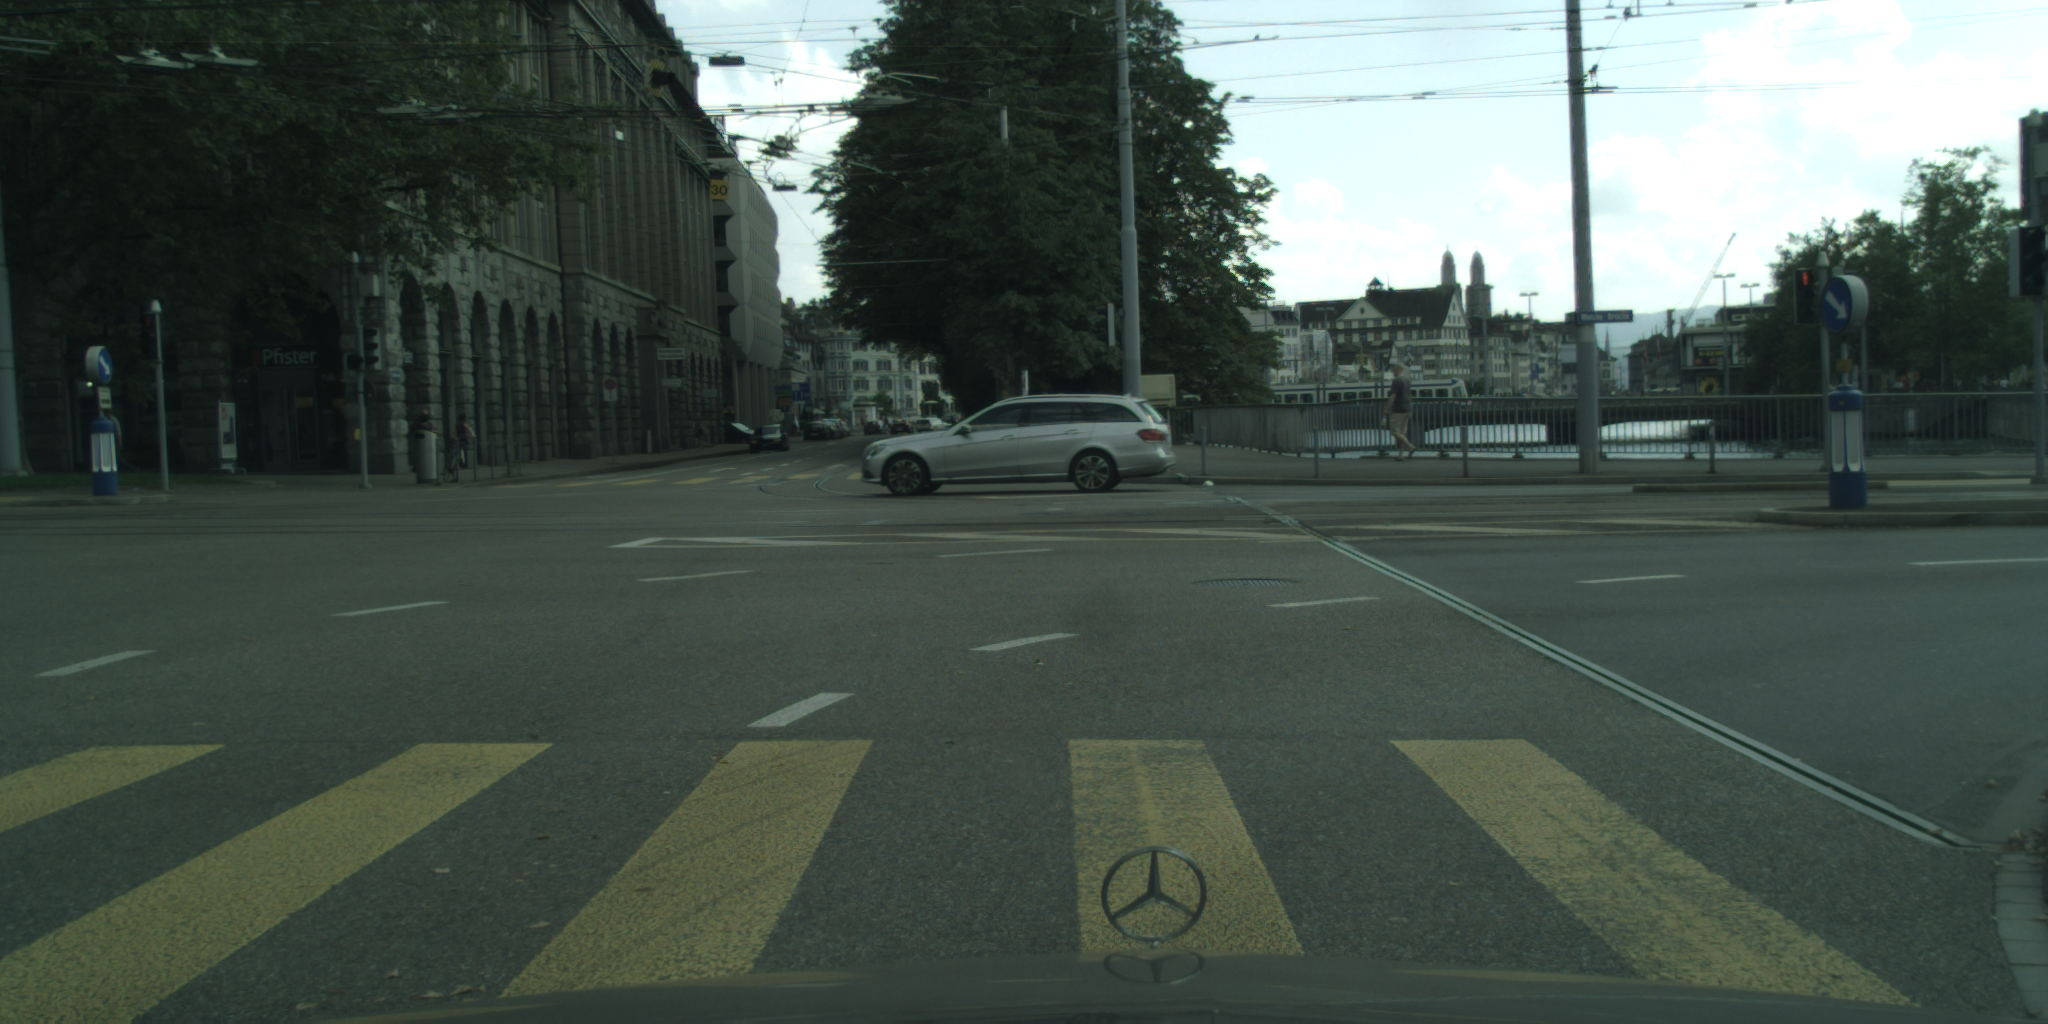
\includegraphics[width=0.35\textwidth]{bad_case.png}
	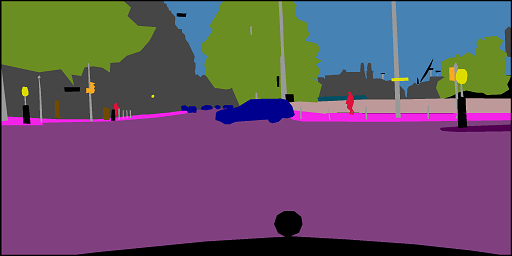
\includegraphics[width=0.35\textwidth]{bad_case_gt.png}
	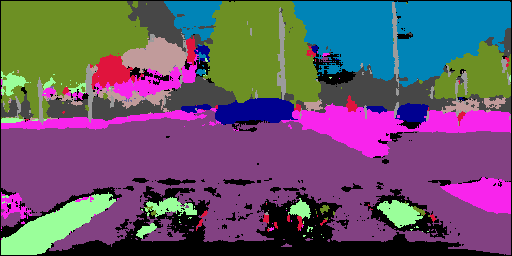
\includegraphics[width=0.35\textwidth]{bad_case_seg.png}
	\caption{Top: input image; middle: ground truth; bottom: segmentation result. We use the network trained with images of size 128$\times$256, and test it on an image of size 256$\times$512. Compared to Figure 5 where the same input image is used but with size 128$\times$256, the output here looks much worse. Therefore, at least for SegNet, performance is influenced by input down-sampling.}
	\label{fig:figure5}
\end{figure}

Since performing segmentation of urban scenes is to reinforce autonomous driving, one can also apply uniform random rotation to each input image and its label, with angle variations from -5 to 5 degrees to simulate vehicle bumping on the road. Intuitively, this method should be able to increase the robustness of real-world applications.


{\small
\bibliographystyle{ieee}
\bibliography{egbib}
}

\end{document}
